Towards simplifying the problem of calculating the contact map overlap measure, an algorithm for computing the same between a staircase and the graph of a self-voiding walk is presented in this section. One can observe that if $T=(V,E)$ is a 2-staircase graph then $E$ can be decomposed into two subsets $E_{1}$ and $E_{2}$ in $O(|E|)$ time where $T_{1}=(V,E_{1})$ and $T_{2}=(V,E_{2})$ are 1-staircase graphs. To understand why this is possible at all, one can consider assigning the edges corresponding to each of the degree 2 nodes of the original staircase $T$ to sets
$E_{1}$ and $E_{2}$ alternatively (Fig. \ref{fig:staircasedecompisition} illustrates this formulation). Since a subgraph of a staircase is also a staircase, both $T_{1}$and $T_{2}$, formed by the above process, become degree $1$ staircase graphs. Therefore, to measure the contact map similarity between a 2-staircase graph and a general graph, it is sufficient to propose algorithm for computing contact map measure between a 1-staircase graph and a general graph.

\begin{figure}[htbp]
\begin{minipage}[b]{0.33\linewidth}
\centering
 \input{staircasedecomp}
 \vspace{0.65cm}
\end{minipage}
\begin{minipage}[b]{0.33\linewidth}
\centering
 \input{staircasedecomp1}
 \vspace{0.65cm}
\end{minipage}
\begin{minipage}[b]{0.33\linewidth}
\centering
 
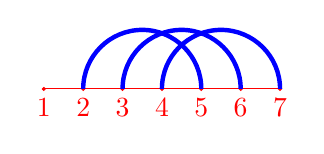
\begin{tikzpicture}[scale=0.5]
\centering
\label{staircasedecompisition}

\foreach \i in {1,...,6} {
        \draw[red] (\i,1) -- (\i + 1,1)node[pos=0.0,below] {\i};
        \filldraw[red] (\i,1) circle (1pt);
 }

\draw[red] (7,1) -- (6,1)node[pos=0.0,below] {7};
\filldraw[red] (7,1) circle (1pt);

\draw[blue, ultra thick] (2,1) arc(180:0:1.5);
\draw[blue, ultra thick] (3,1) arc(180:0:1.5);
\draw[blue, ultra thick] (4,1) arc(180:0:1.5);
\end{tikzpicture}
 \vspace{0.65cm}
\end{minipage}
\caption{A 2-staircase and its decomposition into two 1-staircase}
 \label{fig:staircasedecompisition}
\end{figure}


For further description of the algorithm, the concept of ``cluster" is important which is defined as a set of mutually overlapping edges. From the definition of a staircase graph, it should be obvious that each 1-degree staircase graph consists of only disjoint clusters of edges. Consider one such 1-degree staircase graph $G_1$ consisting of clusters $C_{1}, C_{2}, \cdots, C_{K}$ which is compared to a contact map $G_2=(V_2,E_2)$. Let ${G_1}_{i}$ be the subgraph of $G_1$ consisting of clusters $C_{1}, C_{2}, \cdots, C_{i}$ and ${G_2}_{(1j)}$ be the subgraph of $G_2$ consisting of vertices with indices running from $1$ to $j$ along with the associated edges. A quantity $D(i,j)$ is defined
now to measure the contact map overlap between ${G_1}_{i}$ and ${G_2}_{(1j)}$. The idea is to propose algorithm and measure the complexity for the subgraphs and apply recursion thereafter to compute the similarity measure over the entire graphs.

A consequence of such construction is the following recursive update equation:
\begin{equation}
\label{dim1}
D(i,j) = \max_{0\le r\le m_{i}}\{D(i-1,\Phi(j,r)-1)\} + r,
\end{equation}
where $\Phi(j,r)$ denotes the largest integer $h$ such that ${G_2}_{(hj)}$ contains a cluster of size $r$ as its
subgraph and $m_{i}$ is the number of edges in cluster $C_{i}$.
Let $h^{*}$ denote the largest integer such that ${G_2}_{({h^{*}j})}$ contains $r^{*}$ number of edges obtained from a successful maximal mapping $f^{*}$ between $C_{i}$ and ${G_2}_{({1j})}$. Then, intuitively Eq. \ref{dim1} implies that once one has computed $D(i-1,h^{*}-1)$, the maximum overlap measure between ${G_1}_{(i-1)}$ and ${G_2}_{({(h^{*}-1)j})}$, one can compute $D(i,j)$ by simply solving a maximization problem, assuming $\Phi(j,r)$ is pre-computed. One can see that each step of such recursion takes $O({n_1}_{i})$ time and hence the total computation time is $O(\sum_{{n_1}_{i}}n_2)$ or $O({n_1}{n_2})$.

Pre-computation of $\Phi(j,r)$ can be performed using the following recursive update:
\begin{equation}
\label{rec2}
\Phi(j,r) = \max\{\Phi(j-1,r), \max_{e=(i,j)\in E}\tilde{\Phi}(e,r)\}.
\end{equation}
Here $\tilde{\Phi}(e,r)$ is an auxiliary function corresponding to edge $e\in G_2$ and $r\le {n_2}$ such that $\tilde{\Phi}(e,r)$ is the largest integer $h$ so that ${G_2}_({hj})$ contains a cluster of size $r$ as
its subgraph with $e$ being the rightmost edge of the cluster. Computation of each of such auxiliary functions can be performed in $O({n_2}\log {n_2})$ time according to arguments given in \citet{k73}. Since $G_2$ has $O(n_2)$ edges, total time spent in such computation is $O({n_2}^{2}\log {n_2})$. Combined everything together, the contact map measure between
$G_1$ and $G_2$ can be computed in $O({n_1}{n_2}+{n_2}^{2}\log {n_2})$ time.
